\documentclass{standalone}
\usepackage[dvipsnames]{xcolor}
\usepackage{amsmath}
\usepackage{tikz}
\usetikzlibrary{chains}
\usetikzlibrary{calc}
\usetikzlibrary{shapes}
\usetikzlibrary{shapes.multipart}
\usetikzlibrary{arrows}

\definecolor{webgreen}{rgb}{0,.5,0}
\newcommand{\mstr}[1]{\textup{\color{webgreen}``#1''}}
\newcommand\kk[1]{\textcolor{RoyalBlue}{\text{\textup{\textbf{\texttt{#1}}}}}}
\newcommand\cc[1]{\textcolor{Sepia}{\text{\textup{\textbf{\texttt{#1}}}}}}

\begin{document}

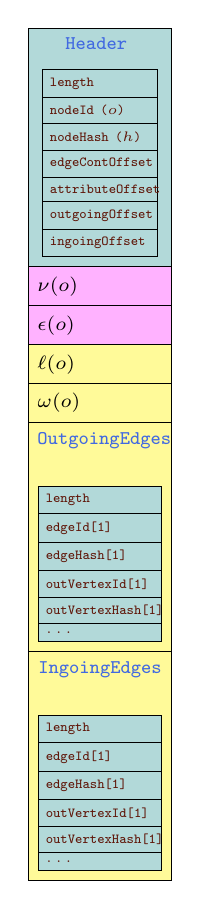
\begin{tikzpicture}
\begin{scope}[start chain=going left,node distance=0pt]
\def\width{9ex}

\tikzstyle{frame}=[
	font=\scriptsize,
	%text width=7ex,
	draw,
	rectangle split,
	rectangle split parts=20,
	rectangle split part align={center, left},
	rectangle split empty part height=0ex,
	rectangle split empty part depth=0ex,
	rectangle split empty part width=0ex,
]

%%MAIN
\node (main) [frame,
	rectangle split parts=7,
	rectangle split part fill={teal!30,Fuchsia!30,Fuchsia!30,yellow!40} 
] {%
\nodepart{one} 
  \begin{minipage}{15ex} \centering
   \kk{Header} \medskip\\
    \tikz{\node (a) [
    draw,
    font=\tiny,
    text width=12ex,
    rectangle split parts=7,
    rectangle split part fill={teal!30},
    rectangle split part align={left,left,left,left,left,left,left,left},
    rectangle split part fill={teal!30,teal!30,teal!30,teal!30,teal!30} 
  ]{%
    \nodepart{one}   \cc{length}
    \nodepart{two}   \cc{nodeId ($o$)}
    \nodepart{three} \cc{nodeHash ($h$)}
    \nodepart{four}  \cc{edgeContOffset}
    \nodepart{five}  \cc{attributeOffset}
    \nodepart{six}   \cc{outgoingOffset}
    \nodepart{seven} \cc{ingoingOffset}
  };}
  \end{minipage}
\nodepart{two}
	{$\nu(o)$}	
\nodepart{three}
	{$\epsilon(o)$}	
\nodepart{four}
	{$\ell(o)$}	
\nodepart{five}
	{$\omega(o)$}		
\nodepart{six}
  \begin{minipage}{15ex} \centering
\kk{OutgoingEdges} \medskip\\
\tikz{\node (b) [
	draw,
	font=\tiny,
	text width=13ex,
	rectangle split parts=6,
	rectangle split part fill={teal!30},
	rectangle split part align={left,left,left,left,left,left,left,left},
	rectangle split part fill={teal!30,teal!30,teal!30,teal!30,teal!30} 
	]{%
		\nodepart{one}   \cc{length}
		\nodepart{two}   \cc{edgeId[1]}
		\nodepart{three} \cc{edgeHash[1]}
		\nodepart{four}  \cc{outVertexId[1]}
		\nodepart{five}  \cc{outVertexHash[1]}
		\nodepart{six}   \cc{$\dots$}
	};}
\end{minipage}
\nodepart{seven}
\begin{minipage}{15ex} \centering
\kk{IngoingEdges} \medskip\\
\tikz{\node (b) [
	draw,
	font=\tiny,
	text width=13ex,
	rectangle split parts=6,
	rectangle split part fill={teal!30},
	rectangle split part align={left,left,left,left,left,left,left,left},
	rectangle split part fill={teal!30,teal!30,teal!30,teal!30,teal!30} 
	]{%
		\nodepart{one}   \cc{length}
		\nodepart{two}   \cc{edgeId[1]}
		\nodepart{three} \cc{edgeHash[1]}
		\nodepart{four}  \cc{outVertexId[1]}
		\nodepart{five}  \cc{outVertexHash[1]}
		\nodepart{six}   \cc{$\dots$}
	};}
\end{minipage}
%\nodepart{five}	
%  \begin{minipage}{14ex} \centering
%   \kk{Ingoing Array}\\
%    \tikz{\node [
%    draw,
%    text width=12ex,
%    font=\tiny,
%    rectangle split parts=4,
%    rectangle split part fill={teal!30,yellow},
%    rectangle split part align={left,left,left,left}
%  ]{%
%    \nodepart{one} \cc{length}
%    \nodepart{two} \cc{in[1]}
%    \nodepart{three} {$\dots$}
%    \nodepart{four}\cc{in[N]}
%  };}
%  \end{minipage}
%\nodepart{six}	
%  \begin{minipage}{14ex} \centering
%  \kk{Outgoing Array}\\
%  \tikz{\node [
%  	draw,
%  	text width=12ex,,origin=c
%  	font=\tiny,
%  	rectangle split parts=4,
%  	rectangle split part fill={teal!30,yellow},
%  	rectangle split part align={left,left,left,left}
%  	]{%
%    \nodepart{one} \cc{length}
%    \nodepart{two} \cc{out[1]}
%    \nodepart{three} {$\dots$}
%    \nodepart{four}\cc{out[O]}
%  	};}
%  \end{minipage}
};

%% SORT
%\node (sort) [frame,
%	rectangle split parts=3,
%	text width=10ex,
%	rectangle split part fill={Fuchsia!30,Fuchsia!30,brown!30} 
%] at (3,0) {%
%\nodepart{one} Vertex Id
%\nodepart{two} Vertex Hash
%\nodepart{three} 
%\begin{minipage}{\width}
%\centering VertexArray offset
%\end{minipage}
%};
%
%\node (qsort1) [frame,
%	rectangle split parts=2,
%	rectangle split part fill={Fuchsia!30,brown!30} 
%] at (-3,0) {%
%\nodepart{one} \centering Hash
%\nodepart{two} \begin{minipage}{\width}
%Vertex\-Array\\ offset
%\end{minipage}
%};
%\node[above=0 pt of main.north,anchor=south,font=\itshape] {VertexArray};
%\node[above=0 pt of sort.north,anchor=south,font=\itshape] {VertexIndex$_i$};
%\node[above=0 pt of qsort1.north,anchor=south,font=\itshape] {Hash$_j$};


%%%%%%%%%%%%EDGES
%\tikzstyle{bp}=[draw=black,thin,->,opacity=0.5,>=latex,->] 
%\draw[*-latex] let  \p1 = ($(main.two east)!0.1!(main.two) $),
%                    \p3 = ($ (main.five north)!0.75!(main.five east)-(0,1) $)
%	           in 
%               (\x1,\y1) edge [bend left] (\x3,\y3);
%;
%\tikzstyle{bp}=[draw=black,thin,->,opacity=0.5,>=latex,->] 
%\draw[*-latex] let \p1 = ($(main.three east)!0.1!(main.three) $),
%				   \p3 = ($ (main.six north)!0.75!(main.six east)-(0,1) $)
%               in 
%               (\x1,\y1) edge [bend left] (\x3,\y3);
               
%%\draw[bp] let 
%%			\p1 = ($(qsort2.two east)!0.1!(qsort2.two) $),
%%         \p2 =  ($(main.text)+(0,1ex) $),
%%           \p3 = ($ (sort.text split)!0.75!(sort.text split east) +(0ex,0)$)
%%	 in 
%%                (\x1,\y1)-- (\x1,\y2) --(\x3,\y2) -- (\x3,\y3);
%%
%%\draw[bp] let 
%%			\p1 = ($(qsort3.two east)!0.1!(qsort3.two) $),
%%         \p2 =  ($(main.text)+(0,2ex) $),
%%           \p3 = ($ (sort.text split)!0.75!(sort.text split east) +(-1ex,0)$)
%%	 in 
%%                (\x1,\y1)-- (\x1,\y2) --(\x3,\y2) -- (\x3,\y3);
%%;
%%
%%\draw[bp] let 
%%			\p1 = ($(swap.two east)!0.1!(swap.two) $),
%%            \p2 =  ($(main.text)+(0,3ex) $),
%%           \p3 = ($ (sort.text split)!0.75!(sort.text split east) +(-2ex,0)$)
%%	 in b
%%                (\x1,\y1)-> (\x1,\y2) -> (\x3,\y2) -> (\x3,\y3);
%%
%%
%%
%%\draw[bp] let 
%%			\p1 = ($(pivot.two east)!0.1!(pivot.two) $),
%%         \p2 =  ($(main.text)+(0,-2.5ex) $),
%%           \p3 = ($ (qsort3.text split)!0.75!(qsort3.text split east) +(-1ex,0)$)
%%	 in 
%%                (\x1,\y1)-- (\x1,\y2) --(\x3,\y2) -- (\x3,\y3);
%%;
%%
%%\draw[bp] 
%%                ($(sort.two east)!0.5!(sort.two) $) |- (a.south west);
%%;
\end{scope}


%\draw[->] (a.one west) edge [bend right] (main.three  west);
%\draw[->] (a.two west) edge [bend right] (main.four  west);
%%
%%\node[above=22pt of main,font=\small,xshift=-30ex]{\textbf{Frames on the hardware stac}};
%%\node[above=10pt of main,font=\footnotesize,xshift=-30ex]{\textit{(grows from high memory to low memory, depicted right to left)}};
\end{tikzpicture}
\end{document}